\documentclass[11pt, a4paper]{article}
\usepackage[utf8]{inputenc}
\usepackage[spanish]{babel}
\usepackage{amsmath, amssymb, amsfonts}
\usepackage{graphicx}
\usepackage{geometry}
\geometry{left=2.5cm, right=2.5cm, top=2.5cm, bottom=2.5cm}
\usepackage{tikz}
\usepackage{bm}
\usepackage[hidelinks]{hyperref}
\graphicspath{{figs/}{../figs/}}


\title{\vspace{-1.5cm}\textbf{Resolución de Ecuaciones Diferenciales Ordinarias}\\ \large Métodos Matemáticos I --- Hoja 2}
\author{\textbf{César Endris Acosta}}

\date{28 de septiembre de 2026}
\begin{document}

\maketitle
\vspace{-0.2cm}

\begin{center}
\fbox{\parbox{0.93\linewidth}{\small
\textbf{Versión interactiva.} Todos los problemas de esta hoja se pueden visualizar e interactuar con sus gráficas
(constantes con deslizadores, curva elegida, campos de direcciones, etc.) en la página web
(pestaña ``Hoja 2''):\\[2pt]
\centerline{\url{https://endris10.github.io/Mathematical_Methods_1/}}\vspace{2pt}
Se utilizó IA (Claude, de Anthropic) \textbf{únicamente para programar la página web};
la resolución de las ecuaciones diferenciales es propia.}}
\end{center}

\noindent\textbf{1. Integrad la EDO: $\bm{8x+4y+1+(4x+2y+1)y^{\prime}=0}$} \\
$z = 4x+2y \implies z' = 4+2y' \implies y' = \dfrac{z'-4}{2}$.
\begin{align*}
2z+1 + (z+1)\frac{z'-4}{2} &= 0 \implies 2(2z+1) + (z+1)(z'-4) = 0 \\
4z+2 + (z+1)z' - 4z - 4 &= 0 \implies (z+1)z' = 2 \implies (z+1)dz = 2dx
\end{align*}
\begin{align*}
\int (z+1)dz &= \int 2dx \implies \frac{1}{2}z^2 + z = 2x + C_1 \implies z^2 + 2z = 4x + C
\end{align*}
\begin{align*}
(4x+2y)^2 + 2(4x+2y) &= 4x + C \implies 16x^2 + 16xy + 4y^2 + 8x + 4y = 4x + C
\end{align*}
\[
\boxed{(4x+2y)^2 + 4x + 4y = C}
\]



\begin{center}
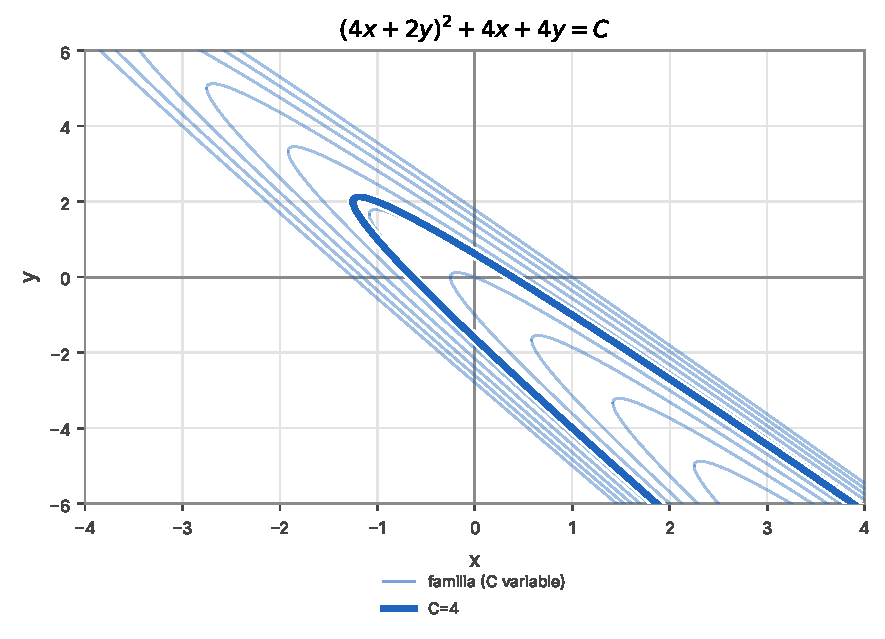
\includegraphics[width=0.8\linewidth]{h2-01.pdf}
\end{center}

\noindent\textbf{2. Integrad la EDO: $\bm{(x-2y-1)dx+(3x-6y+2)dy=0}$} \\
$z = x-2y \implies dx = dz + 2dy$.
\begin{align*}
(z-1)(dz + 2dy) + (3z+2)dy &= 0 \implies (z-1)dz + (2z-2+3z+2)dy = 0 \\
(z-1)dz + 5z\,dy &= 0 \implies \left(1 - \frac{1}{z}\right)dz = -5dy
\end{align*}
\textit{Al dividir por $z$ se excluye $z=0$, es decir $x-2y=0 \implies x=2y \implies dx=2dy$. Sustituyendo $(-1)(2dy) + 2dy = 0$, luego $x-2y=0$ es solución.}
\begin{align*}
\int \left(1 - \frac{1}{z}\right)dz &= \int -5dy \implies z - \ln|z| = -5y + C_1 \\
(x-2y) - \ln|x-2y| &= -5y + C_1 \implies x + 3y - \ln|x-2y| = C_1
\end{align*}
$\implies x-2y = \pm K e^{x+3y}$ con $K>0$; $K\geq 0$ incluye la $x=2y$.
\[
\boxed{x - 2y = \pm K e^{x+3y}, \qquad K \geq 0}
\]



\begin{center}
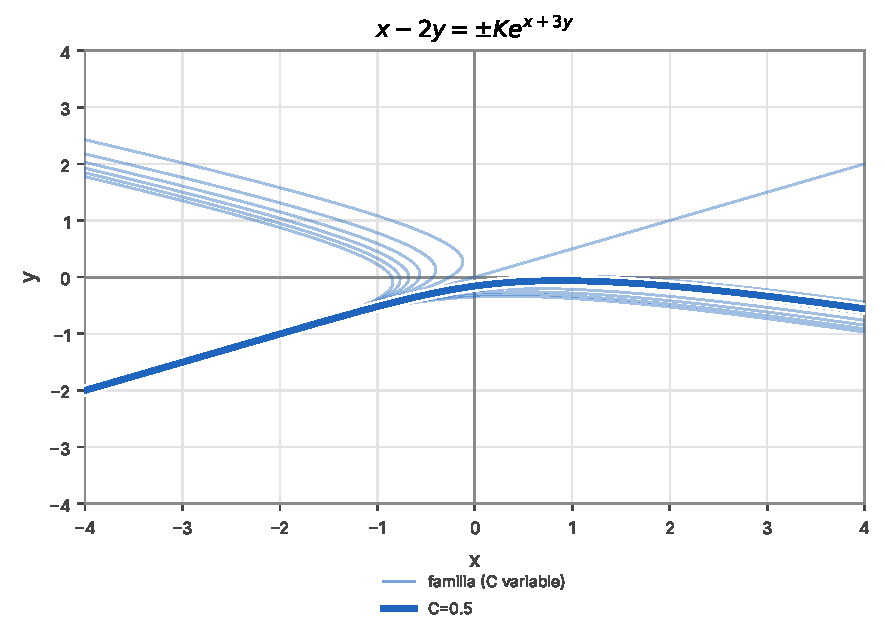
\includegraphics[width=0.8\linewidth]{h2-02.pdf}
\end{center}

\noindent\textbf{3. Integrad la EDO: $\bm{y^{\prime}+2y=e^{-x}}$} \\
\begin{align*}
y'_h + 2y_h &= 0 \implies \frac{dy_h}{y_h} = -2\,dx \implies \ln|y_h| = -2x + C_1 \implies y_h(x) = K e^{-2x}
\end{align*}
$y(x) = C(x) e^{-2x} \implies y' = C'(x) e^{-2x} - 2C(x) e^{-2x}$. \\
\begin{align*}
C'(x) e^{-2x} - 2C(x) e^{-2x} + 2C(x) e^{-2x} &= e^{-x} \implies C'(x) e^{-2x} = e^{-x} \implies C'(x) = e^x \\
C(x) &= \int e^x dx = e^x + C
\end{align*}
\[
\boxed{y(x) = e^{-x} + C e^{-2x}}
\]



\begin{center}
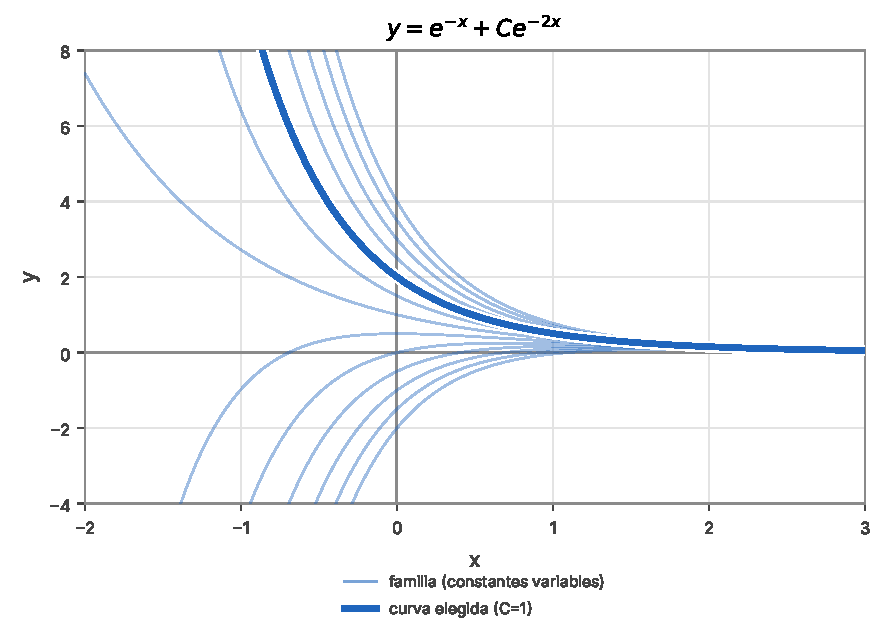
\includegraphics[width=0.8\linewidth]{h2-03.pdf}
\end{center}

\noindent\textbf{4. Integrad la EDO: $\bm{x^{2}+xy^{\prime}=y}$ con la condición inicial $\bm{y(x=1)=0}$} \\
$y' - \frac{1}{x}y = -x$. \\
\begin{align*}
y'_h - \frac{1}{x}y_h &= 0 \implies \frac{dy_h}{y_h} = \frac{dx}{x} \implies \ln|y_h| = \ln|x| + C_1 \implies y_h(x) = Kx
\end{align*}
$y(x) = C(x)x \implies y' = C'(x)x + C(x)$. \\
\begin{align*}
C'(x)x + C(x) - \frac{1}{x}C(x)x &= -x \implies C'(x)x = -x \implies C'(x) = -1 \\
C(x) &= -x + C_0 \implies y(x) = (C_0 - x)x = C_0 x - x^2
\end{align*}
\textit{Al dividir por $x$ se excluye $x=0$} \\
$y(1)=0 \implies C_0(1) - 1^2 = 0 \implies C_0 = 1$.
\[
\boxed{y(x) = x - x^2}
\]



\begin{center}
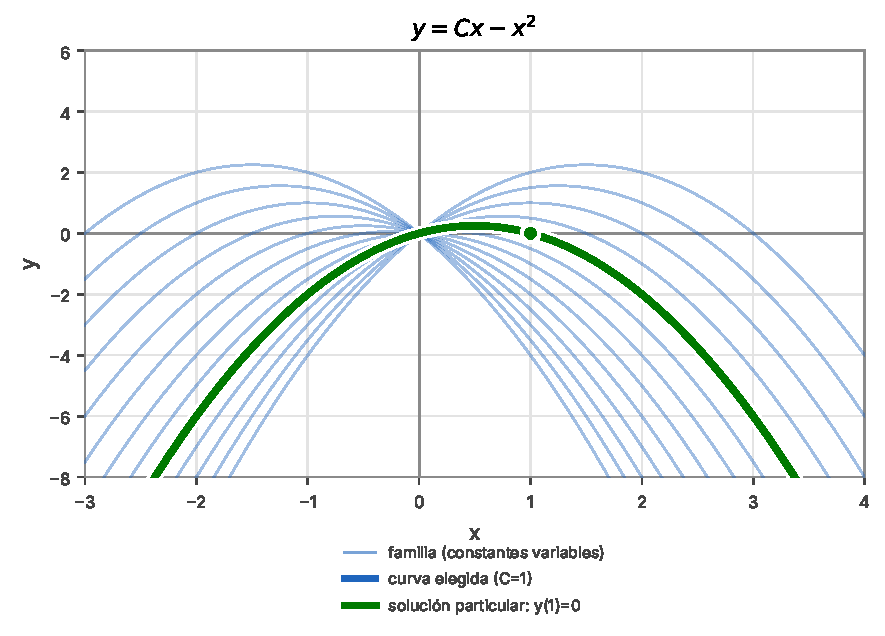
\includegraphics[width=0.8\linewidth]{h2-04.pdf}
\end{center}

\noindent\textbf{5. Integrad la EDO: $\bm{y^{\prime}\cos x-y\sin x=2x}$ con la condición inicial $\bm{y(x=0)=0}$} \\
Dividiendo por $\cos x$: $y' - y\tan x = \frac{2x}{\cos x}$. \\
\begin{align*}
y'_h - y_h\tan x &= 0 \implies \frac{dy_h}{y_h} = \tan x\,dx \implies \ln|y_h| = -\ln|\cos x| + C_1 \implies y_h(x) = K\sec x
\end{align*}
$y(x) = C(x)\sec x \implies y' = C'(x)\sec x + C(x)\sec x\tan x$. \\
Sustituyendo en $y'\cos x - y\sin x = 2x$:
\begin{align*}
\big(C'(x)\sec x + C(x)\sec x\tan x\big)\cos x - C(x)\sec x\sin x &= 2x \implies C'(x) = 2x \\
C(x) &= x^2 + C_0 \implies y(x) = (x^2 + C_0)\sec x
\end{align*}
\textit{La EDO presenta singularidades en $x = \frac{\pi}{2} + k\pi$ donde $\cos x = 0$.} \\
$y(0)=0 \implies (0^2 + C_0)\sec(0) = 0 \implies C_0 = 0$.
\[
\boxed{y(x) = x^2 \sec x}
\]



\begin{center}
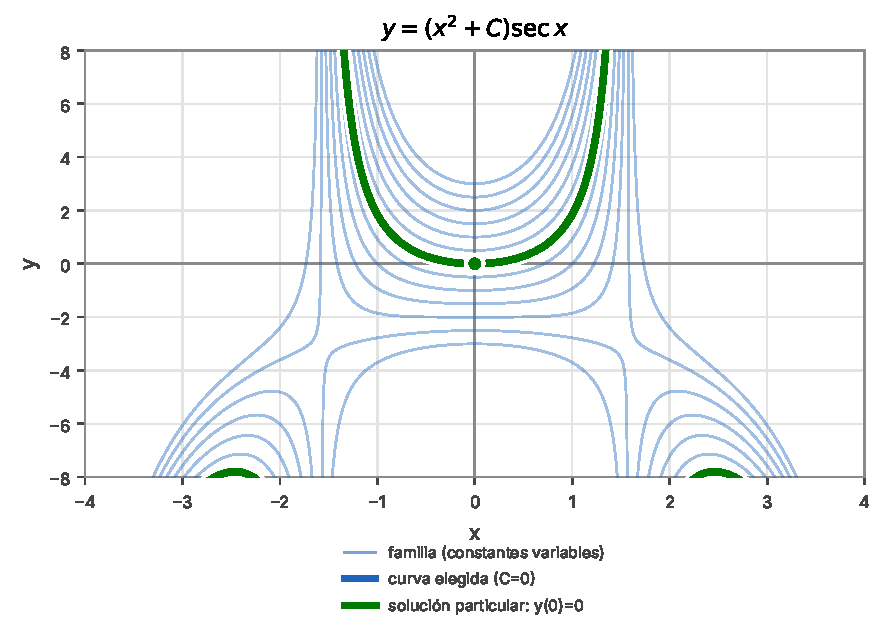
\includegraphics[width=0.8\linewidth]{h2-05.pdf}
\end{center}

\noindent\textbf{6. Integrad la EDO: $\bm{xy^{\prime}-2y=x^{3}\cos x}$} \\
$y' - \frac{2}{x}y = x^2 \cos x$. \\
\begin{align*}
y'_h - \frac{2}{x}y_h &= 0 \implies \frac{dy_h}{y_h} = \frac{2}{x}dx \implies \ln|y_h| = 2\ln|x| + C_1 \implies y_h(x) = Kx^2
\end{align*}
$y(x) = C(x)x^2 \implies y' = C'(x)x^2 + 2C(x)x$. \\
\begin{align*}
x\big(C'(x)x^2 + 2C(x)x\big) - 2C(x)x^2 &= x^3 \cos x \implies C'(x)x^3 = x^3 \cos x \implies C'(x) = \cos x \\
C(x) &= \sin x + C_0 \implies y(x) = (\sin x + C_0)x^2
\end{align*}
\textit{$y=0$ es solución.}
\[
\boxed{y(x) = x^2 \sin x + C x^2}
\]



\begin{center}
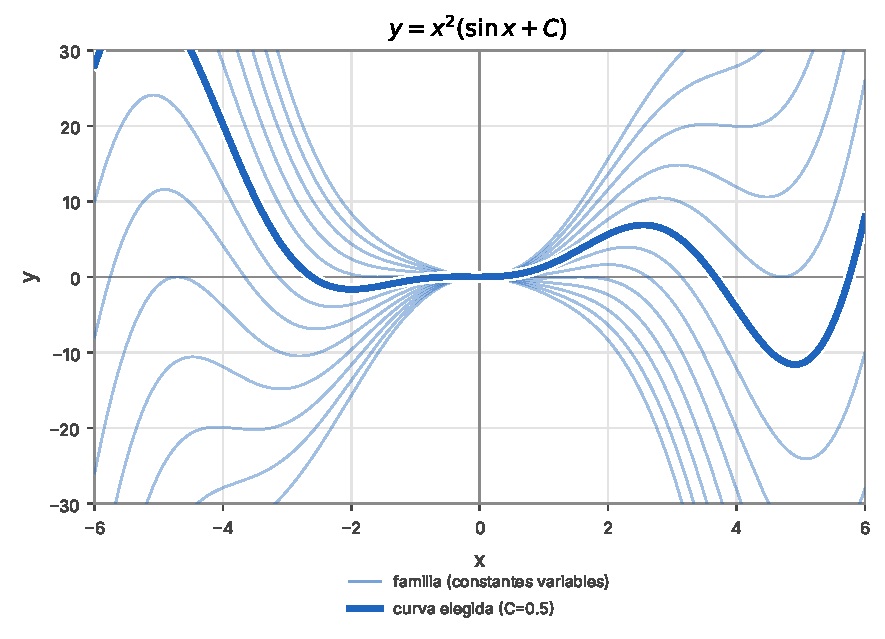
\includegraphics[width=0.8\linewidth]{h2-06.pdf}
\end{center}

\noindent\textbf{7. Integrad la EDO: $\bm{(2x-y^{2})y^{\prime}=2y}$} \\
$P(x,y)dx + N(x,y)dy = 0$:
\begin{align*}
-2y\,dx + (2x-y^2)dy &= 0 \implies P(x,y) = -2y, \quad N(x,y) = 2x-y^2
\end{align*}
\begin{align*}
\frac{\partial P}{\partial y} = -2 \neq \frac{\partial N}{\partial x} = 2 \implies \text{No es exacta.}
\end{align*}
$\mu(y)$:
\begin{align*}
\frac{\frac{\partial N}{\partial x} - \frac{\partial P}{\partial y}}{P} = \frac{2 - (-2)}{-2y} = -\frac{2}{y} \implies \mu(y) = e^{\int -\frac{2}{y}dy} = e^{-2\ln|y|} = \frac{1}{y^2}
\end{align*}
\begin{align*}
-\frac{2}{y}dx + \left(\frac{2x}{y^2} - 1\right)dy &= 0
\end{align*}
Comprobación enla nueva EDO:
\begin{align*}
\tilde{P}(x,y) = -\frac{2}{y} \implies \frac{\partial \tilde{P}}{\partial y} = \frac{2}{y^2}, \qquad \tilde{N}(x,y) = \frac{2x}{y^2} - 1 \implies \frac{\partial \tilde{N}}{\partial x} = \frac{2}{y^2} \quad
\end{align*}
\begin{align*}
F(x,y) &= \int \tilde{P}(x,y) dx = \int -\frac{2}{y}dx = -\frac{2x}{y} + g(y) \\
\frac{\partial F}{\partial y} &= \frac{2x}{y^2} + g'(y) = \tilde{N}(x,y) = \frac{2x}{y^2} - 1 \implies g'(y) = -1 \implies g(y) = -y
\end{align*}
La solución implícita $F(x,y) = C_1$ es:
\begin{align*}
-\frac{2x}{y} - y = C_1 \implies 2x + y^2 = Ky
\end{align*}
\textit{Al dividir por $y^2$ para el factor integrante se excluye $y=0$. Sustituyendo $y\equiv 0$ ($y'=0$) en la EDO original: $(2x-0)\cdot 0 = 2(0)$ se cumple $\forall x$, luego $y=0$ es solución, recuperada con $K=0$.}
\[
\boxed{2x + y^2 = Ky}
\]


\begin{center}
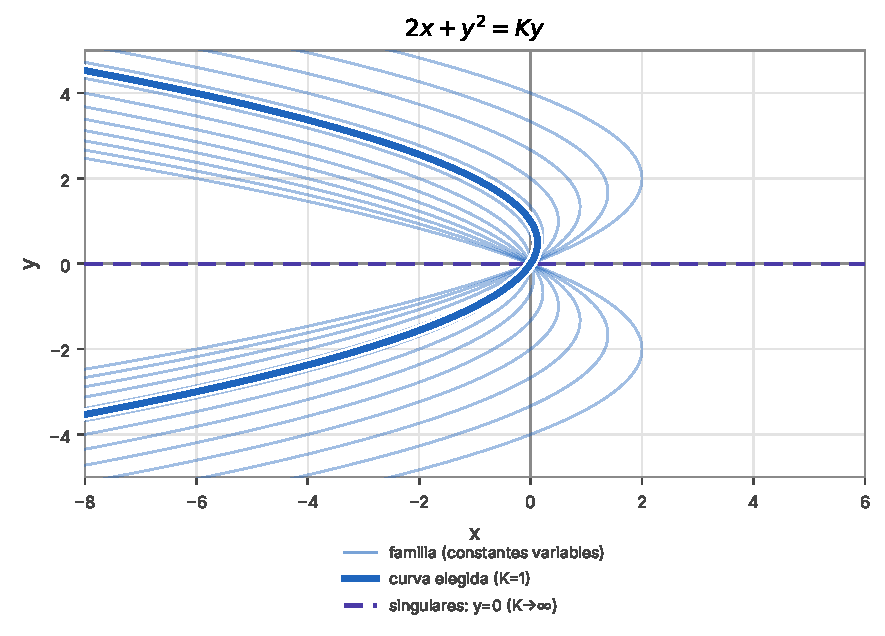
\includegraphics[width=0.8\linewidth]{h2-07.pdf}
\end{center}

\noindent\textbf{8. Integrad la EDO: $\bm{y^{\prime}=\frac{y}{2y\ln y+y-x}}$} \\
$\frac{dx}{dy} + \frac{1}{y}x = 2\ln y + 1$. \\

\begin{align*}
\frac{dx_h}{dy} + \frac{1}{y}x_h &= 0 \implies \frac{dx_h}{x_h} = -\frac{dy}{y} \implies x_h(y) = \frac{C_1}{y}
\end{align*}
$x(y) = \frac{C(y)}{y} \implies \frac{dx}{dy} = \frac{C'(y)y - C(y)}{y^2}$. \\
\begin{align*}
\frac{C'(y)y - C(y)}{y^2} + \frac{C(y)}{y^2} &= 2\ln y + 1 \implies \frac{C'(y)}{y} = 2\ln y + 1 \implies C'(y) = 2y\ln y + y \\
C(y) &= \int (2y\ln y + y)dy = y^2\ln y - \frac{y^2}{2} + \frac{y^2}{2} + K = y^2\ln y + K
\end{align*}
\textit{El dominio pide $y > 0$}
\[
\boxed{x(y) = y\ln y + \frac{K}{y}}
\]



\begin{center}
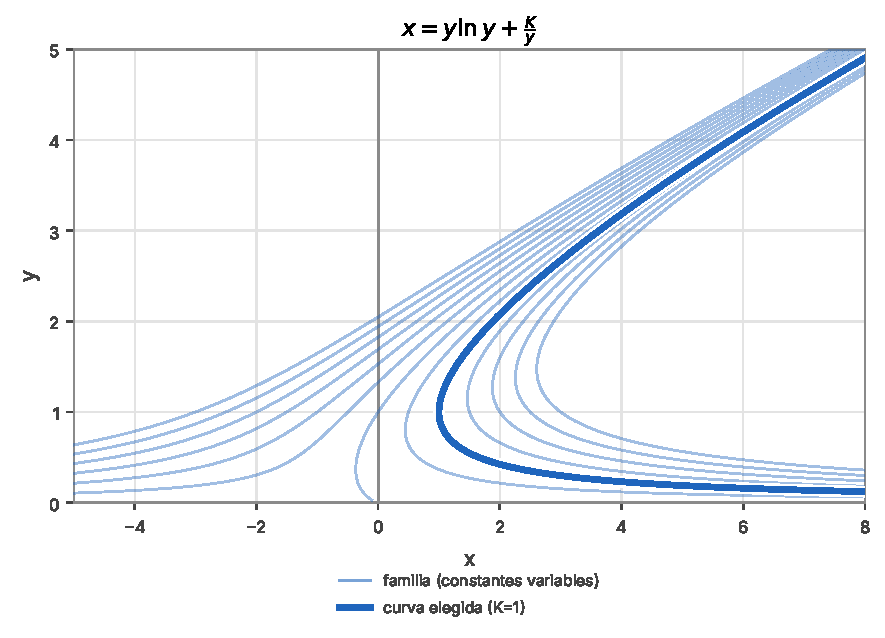
\includegraphics[width=0.8\linewidth]{h2-08.pdf}
\end{center}

\noindent\textbf{9. Integrad la EDO: $\bm{(e^{-y^{2}/2}-xy)dy-dx=0}$} \\
$\frac{dx}{dy} + yx = e^{-y^2/2}$. \\
\begin{align*}
\frac{dx_h}{dy} + yx_h &= 0 \implies \frac{dx_h}{x_h} = -y\,dy \implies x_h(y) = C_1 e^{-y^2/2}
\end{align*}
$x(y) = C(y)e^{-y^2/2} \implies \frac{dx}{dy} = C'(y)e^{-y^2/2} - C(y)y e^{-y^2/2}$. \\
\begin{align*}
C'(y)e^{-y^2/2} - C(y)y e^{-y^2/2} + y C(y)e^{-y^2/2} &= e^{-y^2/2} \implies C'(y) = 1 \implies C(y) = y + C
\end{align*}
\[
\boxed{x e^{y^2/2} - y = C}
\]



\begin{center}
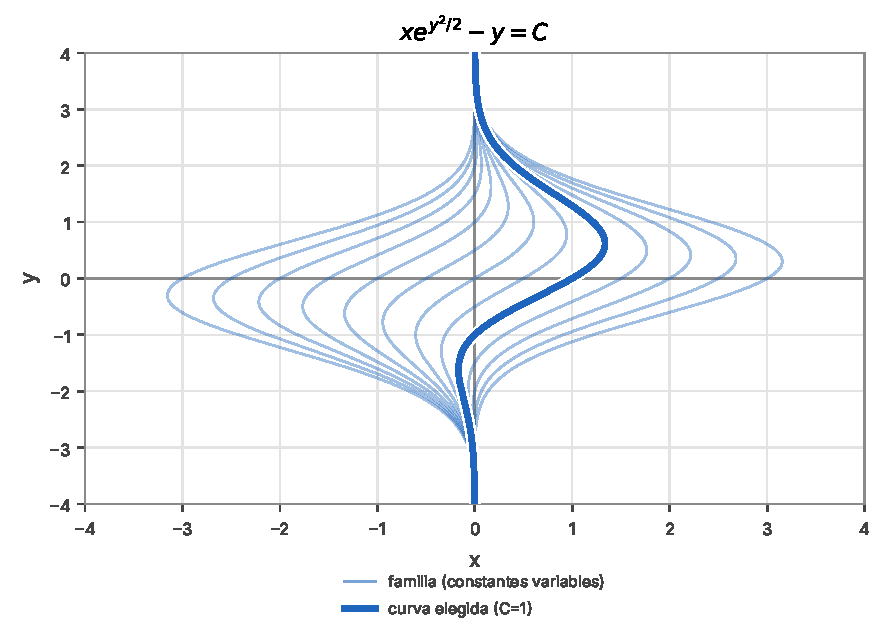
\includegraphics[width=0.8\linewidth]{h2-09.pdf}
\end{center}

\noindent\textbf{10. Integrad la EDO: $\bm{y^{\prime}-y\ln 2=2^{\sin x}(\cos x-1)\ln 2}$ con $\bm{y}$ acotada cuando $\bm{x\rightarrow+\infty}$} \\
\begin{align*}
y'_h - y_h\ln 2 &= 0 \implies \frac{dy_h}{y_h} = \ln 2\,dx \implies y_h(x) = K \cdot 2^x
\end{align*}
$y(x) = C(x) \cdot 2^x \implies y' = C'(x)2^x + C(x)2^x \ln 2$. \\
\begin{align*}
C'(x)2^x + C(x)2^x \ln 2 - C(x)2^x \ln 2 &= 2^{\sin x}(\cos x - 1)\ln 2 \implies C'(x) = 2^{\sin x - x}(\cos x - 1)\ln 2
\end{align*}
$u = \sin x - x \implies du = (\cos x - 1)dx$:
\begin{align*}
C(x) &= \int 2^u \ln 2\,du = 2^u + C_0 = 2^{\sin x - x} + C_0 \implies y(x) = 2^{\sin x} + C_0 \cdot 2^x
\end{align*}

\textit{El término $2^{\sin x}$ está acotado en $[1/2, 2]\ \forall x \in \mathbb{R}$. Analizando la acotación cuando $x \to +\infty$:}
\begin{itemize}
\item \textit{Si $C_0 > 0$, la función cumple acotación por abajo ($y(x) \geq 1/2$), pero diverge a $+\infty$ por arriba.}
\item \textit{Si $C_0 < 0$, cumple acotación superior ($y(x) \leq 2$), pero diverge a $-\infty$ por abajo.}
\item \textit{Por tanto, para asegurar acotación global (tanto superior como inferior) se requiere $C_0 = 0$.}
\end{itemize}
\[
\boxed{y(x) = 2^{\sin x}}
\]



\begin{center}
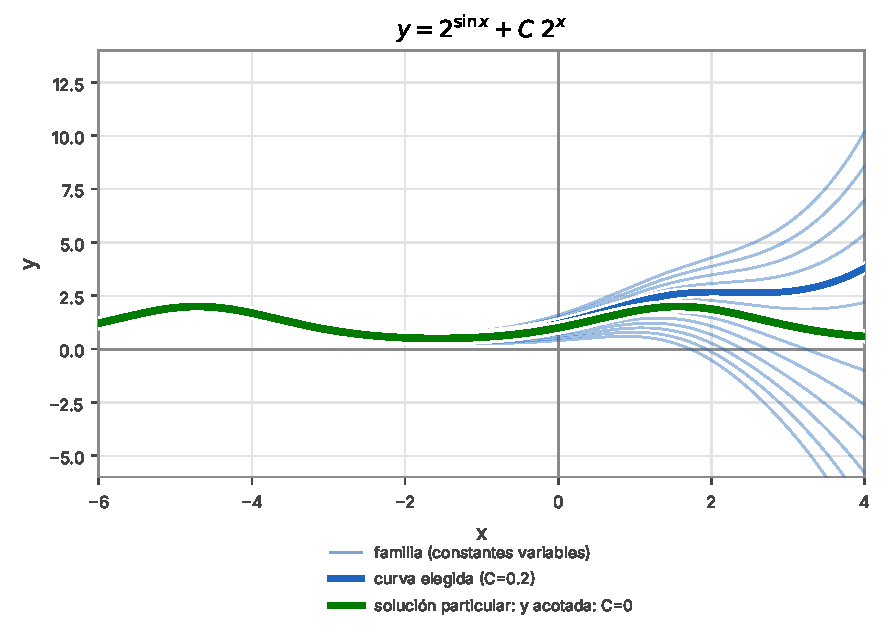
\includegraphics[width=0.8\linewidth]{h2-10.pdf}
\end{center}

\noindent\textbf{11. Integrad la EDO: $\bm{y^{\prime}+2xy=2xy^{2}}$} \\
$z = y^{-1} \implies z' = -y^{-2}y' \implies z' - 2xz = -2x$. \\
\begin{align*}
z'_h - 2xz_h &= 0 \implies \frac{dz_h}{z_h} = 2x\,dx \implies z_h(x) = K e^{x^2}
\end{align*}
$z(x) = C(x)e^{x^2} \implies z' = C'(x)e^{x^2} + 2xC(x)e^{x^2}$. \\
\begin{align*}
C'(x)e^{x^2} + 2xC(x)e^{x^2} - 2xC(x)e^{x^2} &= -2x \implies C'(x) = -2x e^{-x^2} \\
C(x) &= e^{-x^2} + C_0 \implies z(x) = (e^{-x^2} + C_0)e^{x^2} = 1 + C_0 e^{x^2}
\end{align*}
\textit{Al dividir por $y^2$ se excluye $y=0$. $y\equiv 0$ en la EDO original, $0' + 2x(0) = 2x(0)^2$ se satisface $\forall x$, luego $y=0$ es solución (alcanzada para $C_0 \to \infty$).}
\[
\boxed{y(x) = \frac{1}{1 + C e^{x^2}}}
\]



\begin{center}
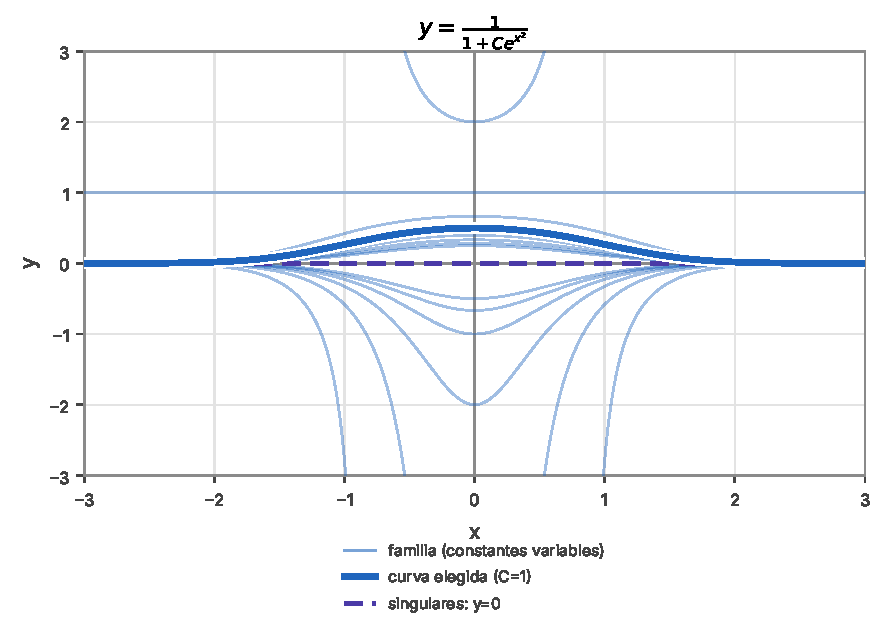
\includegraphics[width=0.8\linewidth]{h2-11.pdf}
\end{center}

\noindent\textbf{12. Integrad la EDO: $\bm{(x^{3}+e^{y})y^{\prime}=3x^{2}}$} \\
$3x^2 \frac{dx}{dy} - x^3 = e^y$. \\
$z = x^3 \implies \frac{dz}{dy} = 3x^2 \frac{dx}{dy} \implies \frac{dz}{dy} - z = e^y$. \\
\begin{align*}
\frac{dz_h}{dy} - z_h &= 0 \implies \frac{dz_h}{z_h} = dy \implies z_h(y) = K e^y
\end{align*}
$z(y) = C(y)e^y \implies \frac{dz}{dy} = C'(y)e^y + C(y)e^y$. \\
\begin{align*}
C'(y)e^y + C(y)e^y - C(y)e^y &= e^y \implies C'(y) = 1 \implies C(y) = y + C_0 \\
z(y) &= (y + C_0)e^y \implies x^3 = (y + C_0)e^y
\end{align*}
\[
\boxed{x^3 = (y+C)e^y}
\]


\begin{center}
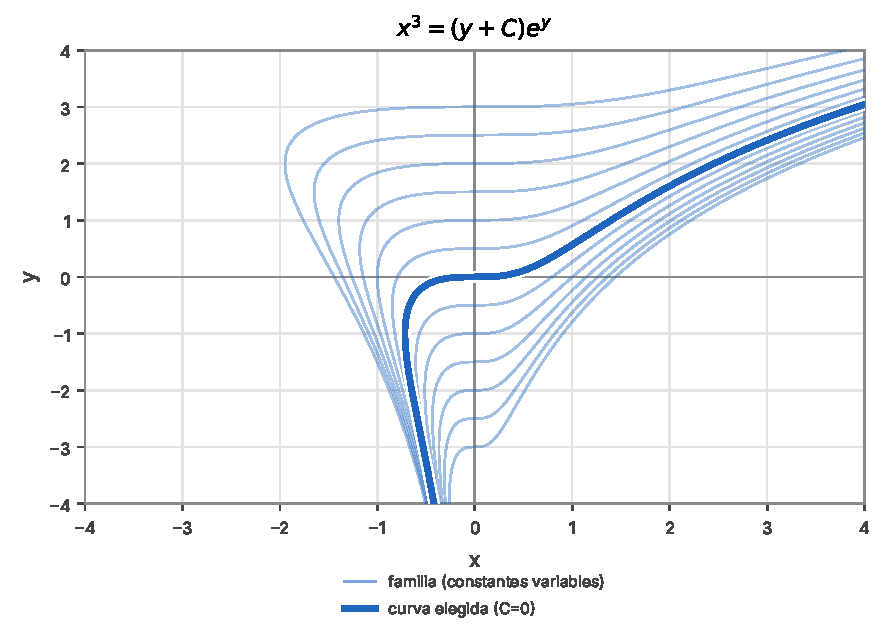
\includegraphics[width=0.8\linewidth]{h2-12.pdf}
\end{center}

\noindent\textbf{13. Integrad la EDO: $\bm{y^{\prime}-2ye^{x}=2\sqrt{y}e^{x}}$} \\
$n=1/2$. $z = \sqrt{y} \implies z' = \frac{1}{2}y^{-1/2}y' \implies z' - z e^x = e^x$. \\
\begin{align*}
z'_h - z_h e^x &= 0 \implies \frac{dz_h}{z_h} = e^x dx \implies z_h(x) = K e^{e^x}
\end{align*}
$z(x) = C(x)e^{e^x} \implies z' = C'(x)e^{e^x} + C(x)e^x e^{e^x}$. \\
\begin{align*}
C'(x)e^{e^x} + C(x)e^x e^{e^x} - C(x)e^x e^{e^x} &= e^x \implies C'(x) = e^x e^{-e^x} \\
C(x) &= -e^{-e^x} + C_0 \implies z(x) = (C_0 - e^{-e^x})e^{e^x} = C_0 e^{e^x} - 1
\end{align*}
\textit{Al dividir por $\sqrt{y}$ se excluye $y=0$; $y\equiv 0$ es solución. Como $z = \sqrt{y} \geq 0$, exige la restricción $C e^{e^x} \geq 1$.}
\[
\boxed{y(x) = \left(C e^{e^x} - 1\right)^2, \qquad C e^{e^x} \geq 1}
\]



\begin{center}
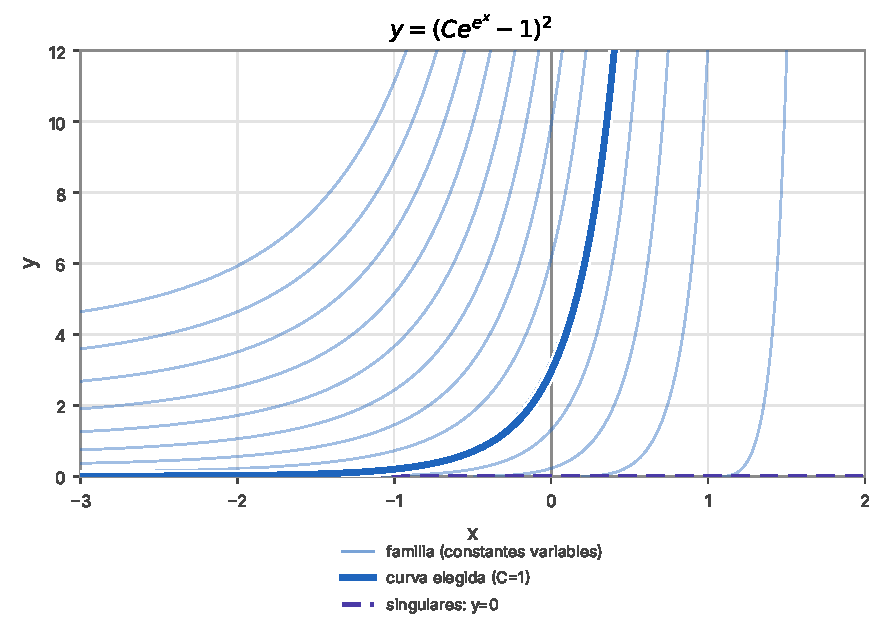
\includegraphics[width=0.8\linewidth]{h2-13.pdf}
\end{center}

\noindent\textbf{14. Integrad la EDO: $\bm{2y^{\prime}\ln x+\frac{y}{x}=\frac{\cos x}{y}}$} \\
$2y y' \ln x + \frac{y^2}{x} = \cos x$. \\
$z = y^2 \implies z' = 2y y' \implies z' \ln x + \frac{z}{x} = \cos x$. \\
\begin{align*}
z'_h \ln x + \frac{z_h}{x} &= 0 \implies \frac{dz_h}{z_h} = -\frac{dx}{x\ln x} \implies \ln|z_h| = -\ln|\ln x| + C_1 \implies z_h(x) = \frac{K}{\ln x}
\end{align*}
Proponemos $z(x) = \frac{C(x)}{\ln x} \implies z' = \frac{C'(x)\ln x - C(x)/x}{\ln^2 x}$. \\
Sustituyendo en la EDO reducida:
\begin{align*}
\left(\frac{C'(x)\ln x - C(x)/x}{\ln^2 x}\right)\ln x + \frac{C(x)}{x\ln x} &= \cos x \implies \frac{C'(x)}{\ln x} = \cos x \implies C'(x) = \cos x \\
C(x) &= \sin x + C_0 \implies z(x) = \frac{\sin x + C_0}{\ln x}
\end{align*}
\textit{El dominio requiere $x > 0$, $x \neq 1$. La división por $y$ excluye $y=0$.}
\[
\boxed{y^2 = \frac{\sin x + C}{\ln x}}
\]



\begin{center}
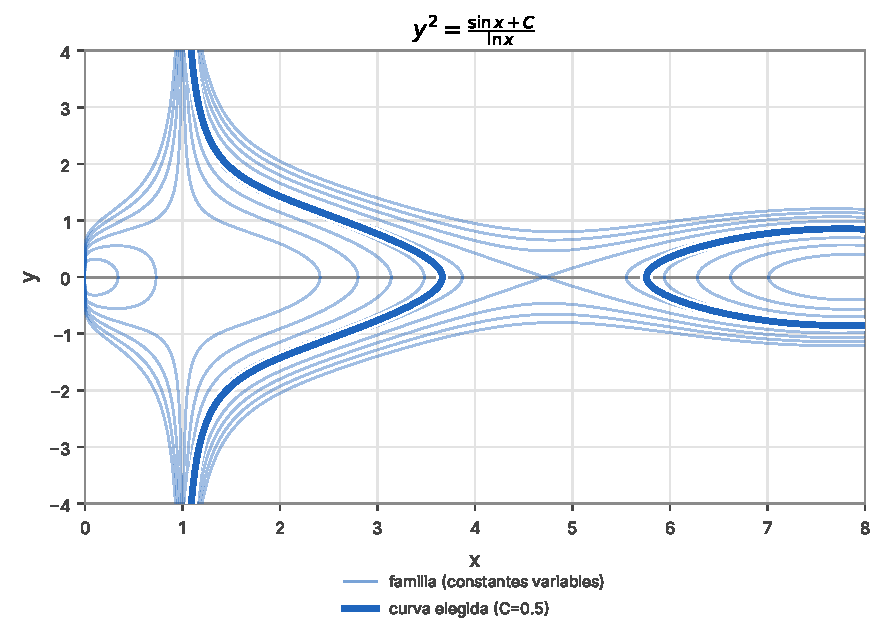
\includegraphics[width=0.8\linewidth]{h2-14.pdf}
\end{center}

\noindent\textbf{15. Integrad la EDO: $\bm{2y^{\prime}\sin x+y\cos x=y^{3}\sin^{2}x}$} \\
Bernoulli con $n=3$. $2y^{-3}y'\sin x + y^{-2}\cos x = \sin^2 x$. \\
$z = y^{-2} \implies z' = -2y^{-3}y' \implies -z'\sin x + z\cos x = \sin^2 x$. \\
\begin{align*}
-z'_h \sin x + z_h \cos x &= 0 \implies \frac{dz_h}{z_h} = \cot x\,dx \implies z_h(x) = K \sin x
\end{align*}
$z(x) = C(x)\sin x \implies z' = C'(x)\sin x + C(x)\cos x$. \\
\begin{align*}
-\big(C'(x)\sin x + C(x)\cos x\big)\sin x + C(x)\sin x\cos x &= \sin^2 x \implies -C'(x)\sin^2 x = \sin^2 x \\
C'(x) &= -1 \implies C(x) = C_0 - x \implies z(x) = (C_0 - x)\sin x
\end{align*}
\textit{Al dividir por $y^3$ se excluye $y=0$, que es solución }
\[
\boxed{y^2 = \frac{1}{(C - x)\sin x}}
\]



\begin{center}
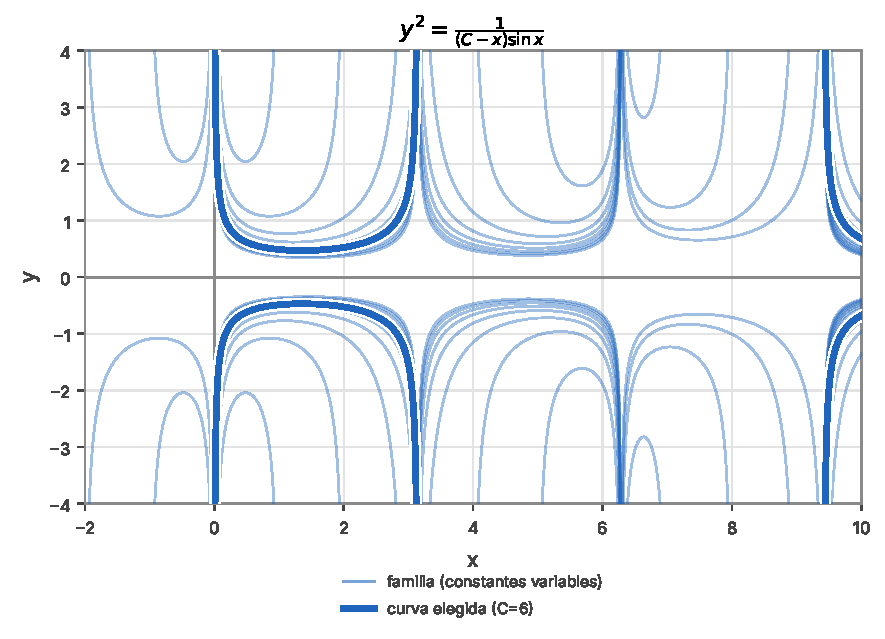
\includegraphics[width=0.8\linewidth]{h2-15.pdf}
\end{center}

\noindent\textbf{16. Resolved mediante derivación la ecuación: $\bm{\int_{0}^{x}ty(t)dt=x^{2}y(x)}$} \\
\begin{align*}
x y(x) &= 2x y(x) + x^2 y'(x) \implies x^2 y'(x) + x y(x) = 0
\end{align*}
Con $x \neq 0$:
\begin{align*}
x y' + y = 0 \implies \frac{dy}{y} = -\frac{dx}{x} \implies \ln|y| = -\ln|x| + C_1
\end{align*}
\[
\boxed{y(x) = \pm\frac{C}{x}, \qquad C>0}
\]



\begin{center}
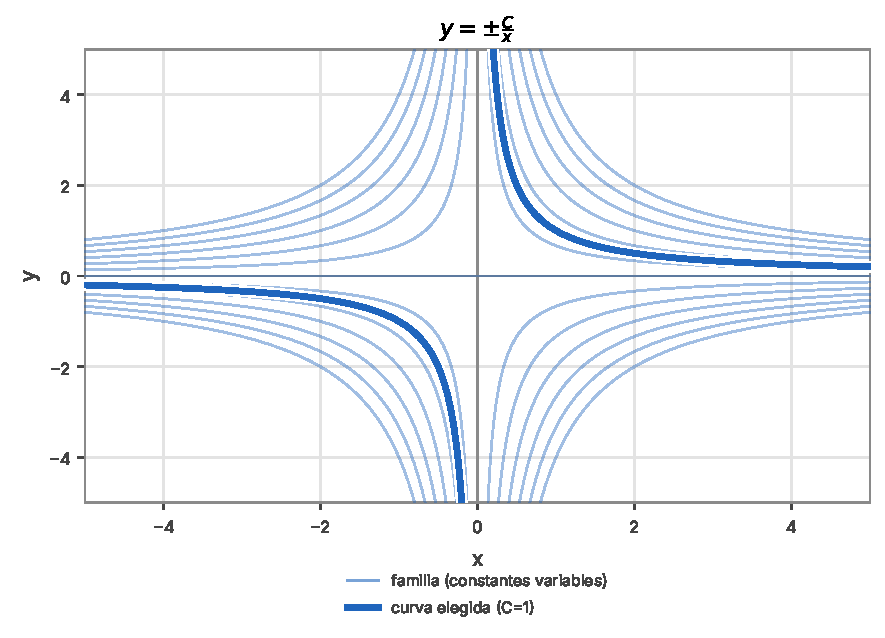
\includegraphics[width=0.8\linewidth]{h2-16.pdf}
\end{center}

\noindent\textbf{17. Resolved mediante derivación la ecuación: $\bm{\int_{0}^{1}y(xt)dt=ny(x)}$} \\
$u = xt \implies du = x\,dt \implies dt = \frac{du}{x}$.\\
$t=0 \to u=0$, $t=1 \to u=x$.
\begin{align*}
\frac{1}{x} \int_{0}^{x} y(u) du &= n y(x) \implies \int_{0}^{x} y(u) du = n x y(x)
\end{align*}
\begin{align*}
y(x) &= n \left[ y(x) + x y'(x) \right] \implies y(x) = n y(x) + n x y'(x) \\
n x y'(x) &= (1-n) y(x) \implies \frac{dy}{y} = \frac{1-n}{n} \frac{dx}{x}
\end{align*}
$\ln|y| = \frac{1-n}{n}\ln|x| + C_1$.
\[
\boxed{y(x) = C x^{\frac{1-n}{n}}}
\]



\begin{center}
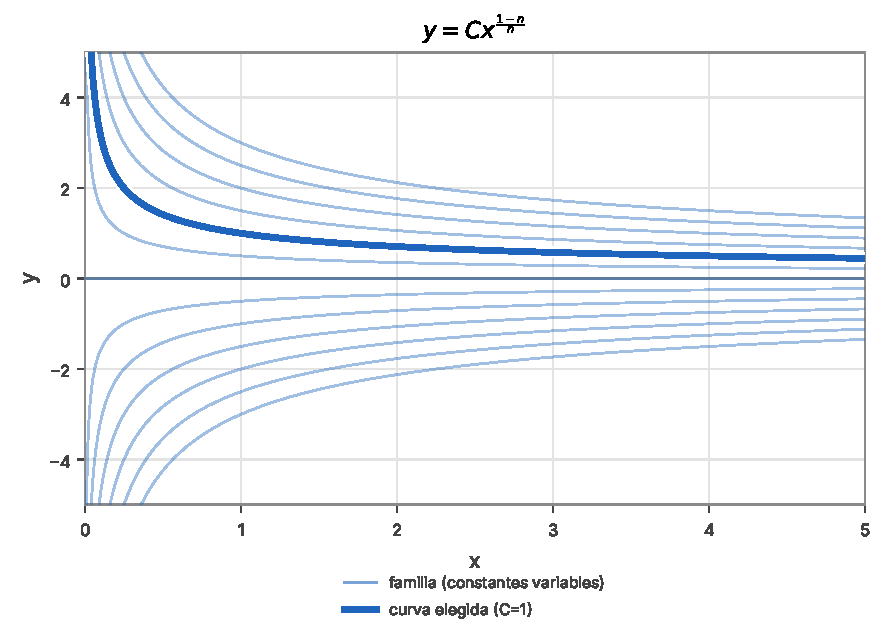
\includegraphics[width=0.8\linewidth]{h2-17.pdf}
\end{center}

\noindent\textbf{18. Integrad la EDO: $\bm{x(2x^{2}+y^{2})+y(x^{2}+2y^{2})y^{\prime}=0}$} \\
$M(x,y)dx + N(x,y)dy = 0$:
\begin{align*}
(2x^3 + xy^2)dx + (x^2y + 2y^3)dy &= 0
\end{align*}
Comprobación de exacta: $\frac{\partial M}{\partial y} = 2xy = \frac{\partial N}{\partial x} \implies \text{Lo es, xd}$. \\
\begin{align*}
f(x,y) &= \int (2x^3 + xy^2)dx = \frac{1}{2}x^4 + \frac{1}{2}x^2y^2 + g(y) \\
\frac{\partial f}{\partial y} &= x^2y + g'(y) = x^2y + 2y^3 \implies g'(y) = 2y^3 \implies g(y) = \frac{1}{2}y^4
\end{align*}
\[
\boxed{x^4 + x^2y^2 + y^4 = C}
\]



\begin{center}
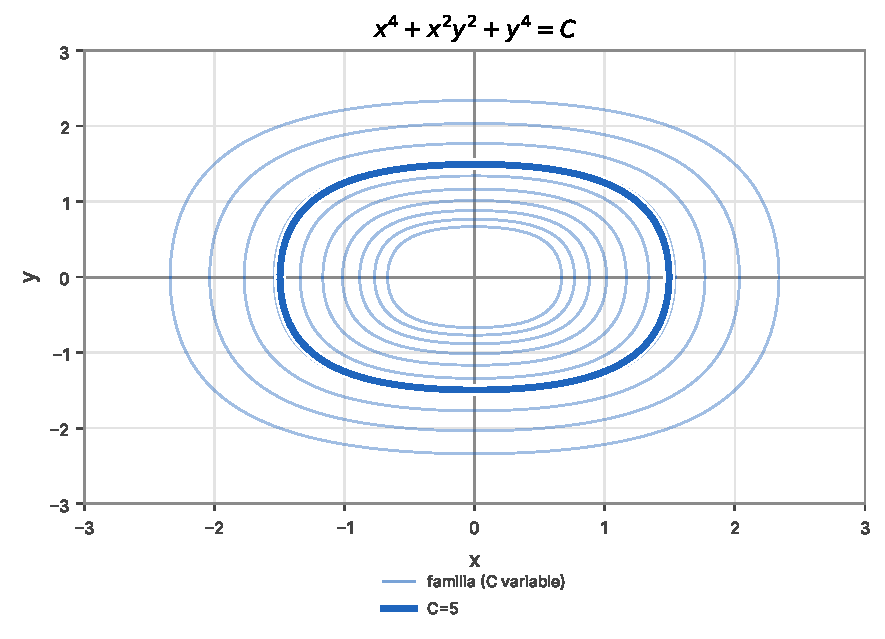
\includegraphics[width=0.8\linewidth]{h2-18.pdf}
\end{center}

\noindent\textbf{19. Integrad la EDO: $\bm{\left(\frac{x}{\sqrt{x^{2}+y^{2}}}+\frac{1}{x}+\frac{1}{y}\right)dx+\left(\frac{y}{\sqrt{x^{2}+y^{2}}}+\frac{1}{y}-\frac{x}{y^{2}}\right)dy=0}$} \\
\begin{align*}
\frac{\partial M}{\partial y} &= -\frac{xy}{(x^2+y^2)^{3/2}} - \frac{1}{y^2}, \qquad \frac{\partial N}{\partial x} = -\frac{xy}{(x^2+y^2)^{3/2}} - \frac{1}{y^2} \implies \text{Es exacta}
\end{align*}
\begin{align*}
f(x,y) &= \int \left(\frac{x}{\sqrt{x^2+y^2}} + \frac{1}{x} + \frac{1}{y}\right) dx = \sqrt{x^2+y^2} + \ln|x| + \frac{x}{y} + g(y) \\
\frac{\partial f}{\partial y} &= \frac{y}{\sqrt{x^2+y^2}} - \frac{x}{y^2} + g'(y) = \frac{y}{\sqrt{x^2+y^2}} + \frac{1}{y} - \frac{x}{y^2} \implies g'(y) = \frac{1}{y} \implies g(y) = \ln|y|
\end{align*}
\textit{El dominio de la EDO requiere $x \neq 0$ y $y \neq 0$.}
\[
\boxed{\sqrt{x^2+y^2} + \ln|xy| + \frac{x}{y} = C}
\]



\begin{center}
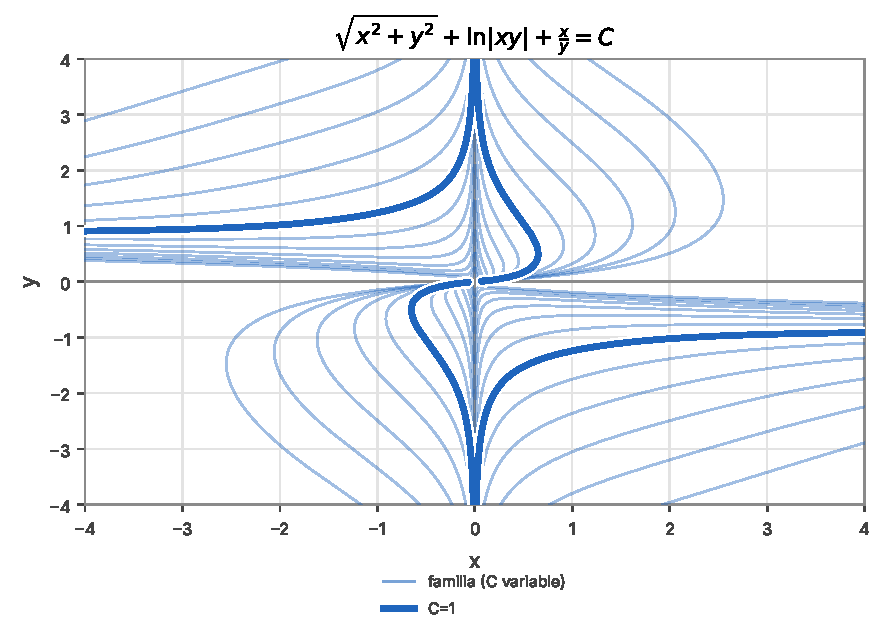
\includegraphics[width=0.8\linewidth]{h2-19.pdf}
\end{center}

\noindent\textbf{20. Integrad la EDO: $\bm{\left(3x^{2}\tan y-\frac{2y^{3}}{x^{3}}\right)dx+\left(x^{3}\sec^{2}y+4y^{3}+\frac{3y^{2}}{x^{2}}\right)dy=0}$} \\
\begin{align*}
\frac{\partial M}{\partial y} &= 3x^2\sec^2 y - \frac{6y^2}{x^3}, \qquad \frac{\partial N}{\partial x} = 3x^2\sec^2 y - \frac{6y^2}{x^3} \implies \text{Otra vez exacta}\\
f(x,y) &= \int \left(3x^2\tan y - \frac{2y^3}{x^3}\right) dx = x^3\tan y + \frac{y^3}{x^2} + g(y) \\
\frac{\partial f}{\partial y} &= x^3\sec^2 y + \frac{3y^2}{x^2} + g'(y) = x^3\sec^2 y + 4y^3 + \frac{3y^2}{x^2} \implies g'(y) = 4y^3 \implies g(y) = y^4
\end{align*}
\textit{El dominio pide $x \neq 0$ y $y \neq \frac{\pi}{2} + k\pi$.}
\[
\boxed{x^3\tan y + \frac{y^3}{x^2} + y^4 = C}
\]


\begin{center}
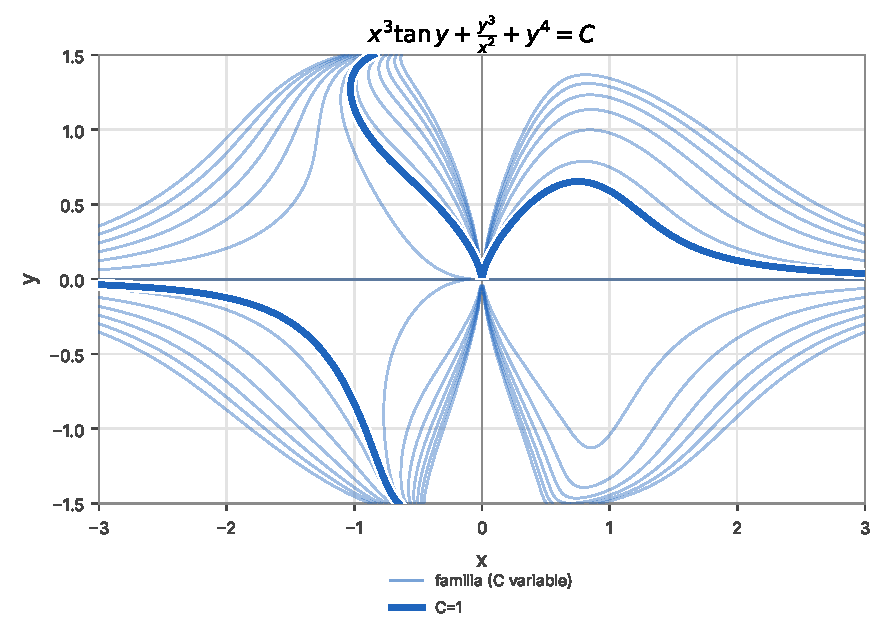
\includegraphics[width=0.8\linewidth]{h2-20.pdf}
\end{center}

\end{document}
